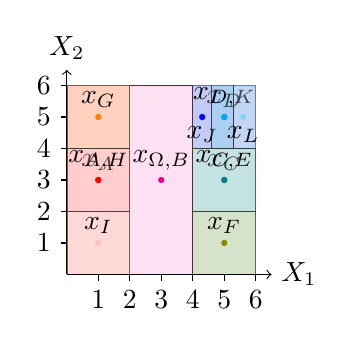
\begin{tikzpicture}[scale=0.4]

    % Define backgroun
     \draw[step=6,black,very thin] (0,0) grid (6,6);    

      % First decomposition : section(space) -> A,B,C
      \draw (2,0) -- (2,6) ;
      \draw (4,0) -- (4,6);
          % define A
          \fill[red!50, opacity = 0.3] (0.0,0) rectangle (2,6);
          % define B
          \fill[magenta!40, opacity = 0.3] (2,0) rectangle (4,6);
          \fill[fill = magenta] (3,3) circle (0.1) node[above]{$x_{\Omega, B}$};   
          % define C
          \fill[teal!50, opacity = 0.3] (4,0) rectangle (6,6);
             
    
    \onslide<1>{
      %define C
      \fill[fill = teal] (5,3) circle (0.1) node[above]{$x_{C}$};
    }
    \onslide<1,2>{
      %define A
      \fill[fill = red] (1,3) circle (0.1) node[above]{$x_A$};
    }
    %%%%%%%%% Second Iteration : D,E,F  %%%%%%
    \onslide<2->{
      % second decomposition : section(C) -> D,E,F
      \draw (4,2) -- (6,2);
      \draw (4,4) -- (6,4);
        % point D
        \fill[blue!50, opacity = 0.3] (4,4) rectangle (6,6);
        %point E
        \fill[teal!40, opacity = 0.3] (4,2) rectangle (6,4);
        \fill[fill = teal] (5,3) circle ( 0.1)node[above]{$x_{C,E}$} ;   
        %point F
        \fill[olive!40, opacity = 0.3] (4,0) rectangle (6,2);
        \fill[fill = olive] (5,1) circle ( 0.1) node[above]{$x_F$} ;  
    } 
    \onslide<2>{
      \fill[fill = blue] (5,5) circle ( 0.1) node[above]{$x_{D}$} ;  
    }

    %%%%%%%%% Second Iteration : G,H,I and J,K,L  %%%%%%
    \onslide<3->{
      % Third decomposition : section(A) -> G,H,I
      \draw (0,2) -- (2,2);
      \draw (0,4) -- (2,4);
        % point G
        \fill[orange!50, opacity = 0.3] (0,4) rectangle (2,6);
        \fill[fill = orange] (1,5) circle ( 0.1) node[above]{$x_{G}$} ;
        %point H
        \fill[red!30, opacity = 0.3] (0,2) rectangle (2,4);
        \fill[fill = red] (1,3) circle ( 0.1)node[above]{$x_{A,H}$};   
        %point F
        \fill[pink!60, opacity = 0.3] (0,0) rectangle (2,2);
        \fill[fill = pink] (1,1) circle ( 0.1) node[above]{$x_I$} ;  

      % Forth decomposition : section(D) -> J,K,L
      \draw (4.6,4) -- (4.6,6);
      \draw (5.3,4) -- (5.3,6);
        %point J
        \fill[blue!20, opacity = 0.3] (4,4) rectangle (4.6,6);
        \fill[fill = blue] (4.3,5) circle ( 0.1) node[below]{$x_J$} ;   
        %point K
        \fill[cyan!50, opacity = 0.3] (4.6,4) rectangle (5.3,6);
        \fill[fill = cyan] (5,5) circle ( 0.1)node[above]{$x_{D,K}$};   
        %point L
        \fill[cyan!20, opacity = 0.3] (5.3,4) rectangle (6,6);
        \fill[fill = cyan!50] (5.6,5) circle ( 0.1) node[below]{$x_L$} ;   
    }

    % Draw red points
    \fill[red] (3,3) circle (0.01);   

    
    % Draw the axes
    \draw[->] (0,0) -- (6.5,0) node[right] {$X_1$};
    \draw[->] (0,0) -- (0,6.5) node[above] {$X_2$};
    
    % Add ticks and labels
    \foreach \x in {1,2,3,4,5,6} {
      \draw (\x,0) -- (\x,-0.2) node[below] {\x};
      \draw (0,\x) -- (-0.2,\x) node[left] {\x};
    }
    
\end{tikzpicture}